\documentclass[1p]{elsarticle_modified}
%\bibliographystyle{elsarticle-num}

%\usepackage[colorlinks]{hyperref}
%\usepackage{abbrmath_seonhwa} %\Abb, \Ascr, \Acal ,\Abf, \Afrak
\usepackage{amsfonts}
\usepackage{amssymb}
\usepackage{amsmath}
\usepackage{amsthm}
\usepackage{scalefnt}
\usepackage{amsbsy}
\usepackage{kotex}
\usepackage{caption}
\usepackage{subfig}
\usepackage{color}
\usepackage{graphicx}
\usepackage{xcolor} %% white, black, red, green, blue, cyan, magenta, yellow
\usepackage{float}
\usepackage{setspace}
\usepackage{hyperref}

\usepackage{tikz}
\usetikzlibrary{arrows}

\usepackage{multirow}
\usepackage{array} % fixed length table
\usepackage{hhline}

%%%%%%%%%%%%%%%%%%%%%
\makeatletter
\renewcommand*\env@matrix[1][\arraystretch]{%
	\edef\arraystretch{#1}%
	\hskip -\arraycolsep
	\let\@ifnextchar\new@ifnextchar
	\array{*\c@MaxMatrixCols c}}
\makeatother %https://tex.stackexchange.com/questions/14071/how-can-i-increase-the-line-spacing-in-a-matrix
%%%%%%%%%%%%%%%

\usepackage[normalem]{ulem}

\newcommand{\msout}[1]{\ifmmode\text{\sout{\ensuremath{#1}}}\else\sout{#1}\fi}
%SOURCE: \msout is \stkout macro in https://tex.stackexchange.com/questions/20609/strikeout-in-math-mode

\newcommand{\cancel}[1]{
	\ifmmode
	{\color{red}\msout{#1}}
	\else
	{\color{red}\sout{#1}}
	\fi
}

\newcommand{\add}[1]{
	{\color{blue}\uwave{#1}}
}

\newcommand{\replace}[2]{
	\ifmmode
	{\color{red}\msout{#1}}{\color{blue}\uwave{#2}}
	\else
	{\color{red}\sout{#1}}{\color{blue}\uwave{#2}}
	\fi
}

\newcommand{\Sol}{\mathcal{S}} %segment
\newcommand{\D}{D} %diagram
\newcommand{\A}{\mathcal{A}} %arc


%%%%%%%%%%%%%%%%%%%%%%%%%%%%%5 test

\def\sl{\operatorname{\textup{SL}}(2,\Cbb)}
\def\psl{\operatorname{\textup{PSL}}(2,\Cbb)}
\def\quan{\mkern 1mu \triangleright \mkern 1mu}

\theoremstyle{definition}
\newtheorem{thm}{Theorem}[section]
\newtheorem{prop}[thm]{Proposition}
\newtheorem{lem}[thm]{Lemma}
\newtheorem{ques}[thm]{Question}
\newtheorem{cor}[thm]{Corollary}
\newtheorem{defn}[thm]{Definition}
\newtheorem{exam}[thm]{Example}
\newtheorem{rmk}[thm]{Remark}
\newtheorem{alg}[thm]{Algorithm}

\newcommand{\I}{\sqrt{-1}}
\begin{document}

%\begin{frontmatter}
%
%\title{Boundary parabolic representations of knots up to 8 crossings}
%
%%% Group authors per affiliation:
%\author{Yunhi Cho} 
%\address{Department of Mathematics, University of Seoul, Seoul, Korea}
%\ead{yhcho@uos.ac.kr}
%
%
%\author{Seonhwa Kim} %\fnref{s_kim}}
%\address{Center for Geometry and Physics, Institute for Basic Science, Pohang, 37673, Korea}
%\ead{ryeona17@ibs.re.kr}
%
%\author{Hyuk Kim}
%\address{Department of Mathematical Sciences, Seoul National University, Seoul 08826, Korea}
%\ead{hyukkim@snu.ac.kr}
%
%\author{Seokbeom Yoon}
%\address{Department of Mathematical Sciences, Seoul National University, Seoul, 08826,  Korea}
%\ead{sbyoon15@snu.ac.kr}
%
%\begin{abstract}
%We find all boundary parabolic representation of knots up to 8 crossings.
%
%\end{abstract}
%\begin{keyword}
%    \MSC[2010] 57M25 
%\end{keyword}
%
%\end{frontmatter}

%\linenumbers
%\tableofcontents
%
\newcommand\colored[1]{\textcolor{white}{\rule[-0.35ex]{0.8em}{1.4ex}}\kern-0.8em\color{red} #1}%
%\newcommand\colored[1]{\textcolor{white}{ #1}\kern-2.17ex	\textcolor{white}{ #1}\kern-1.81ex	\textcolor{white}{ #1}\kern-2.15ex\color{red}#1	}

{\Large $\underline{12a_{0533}~(K12a_{0533})}$}

\setlength{\tabcolsep}{10pt}
\renewcommand{\arraystretch}{1.6}
\vspace{1cm}\begin{tabular}{m{100pt}>{\centering\arraybackslash}m{274pt}}
\multirow{5}{120pt}{
	\centering
	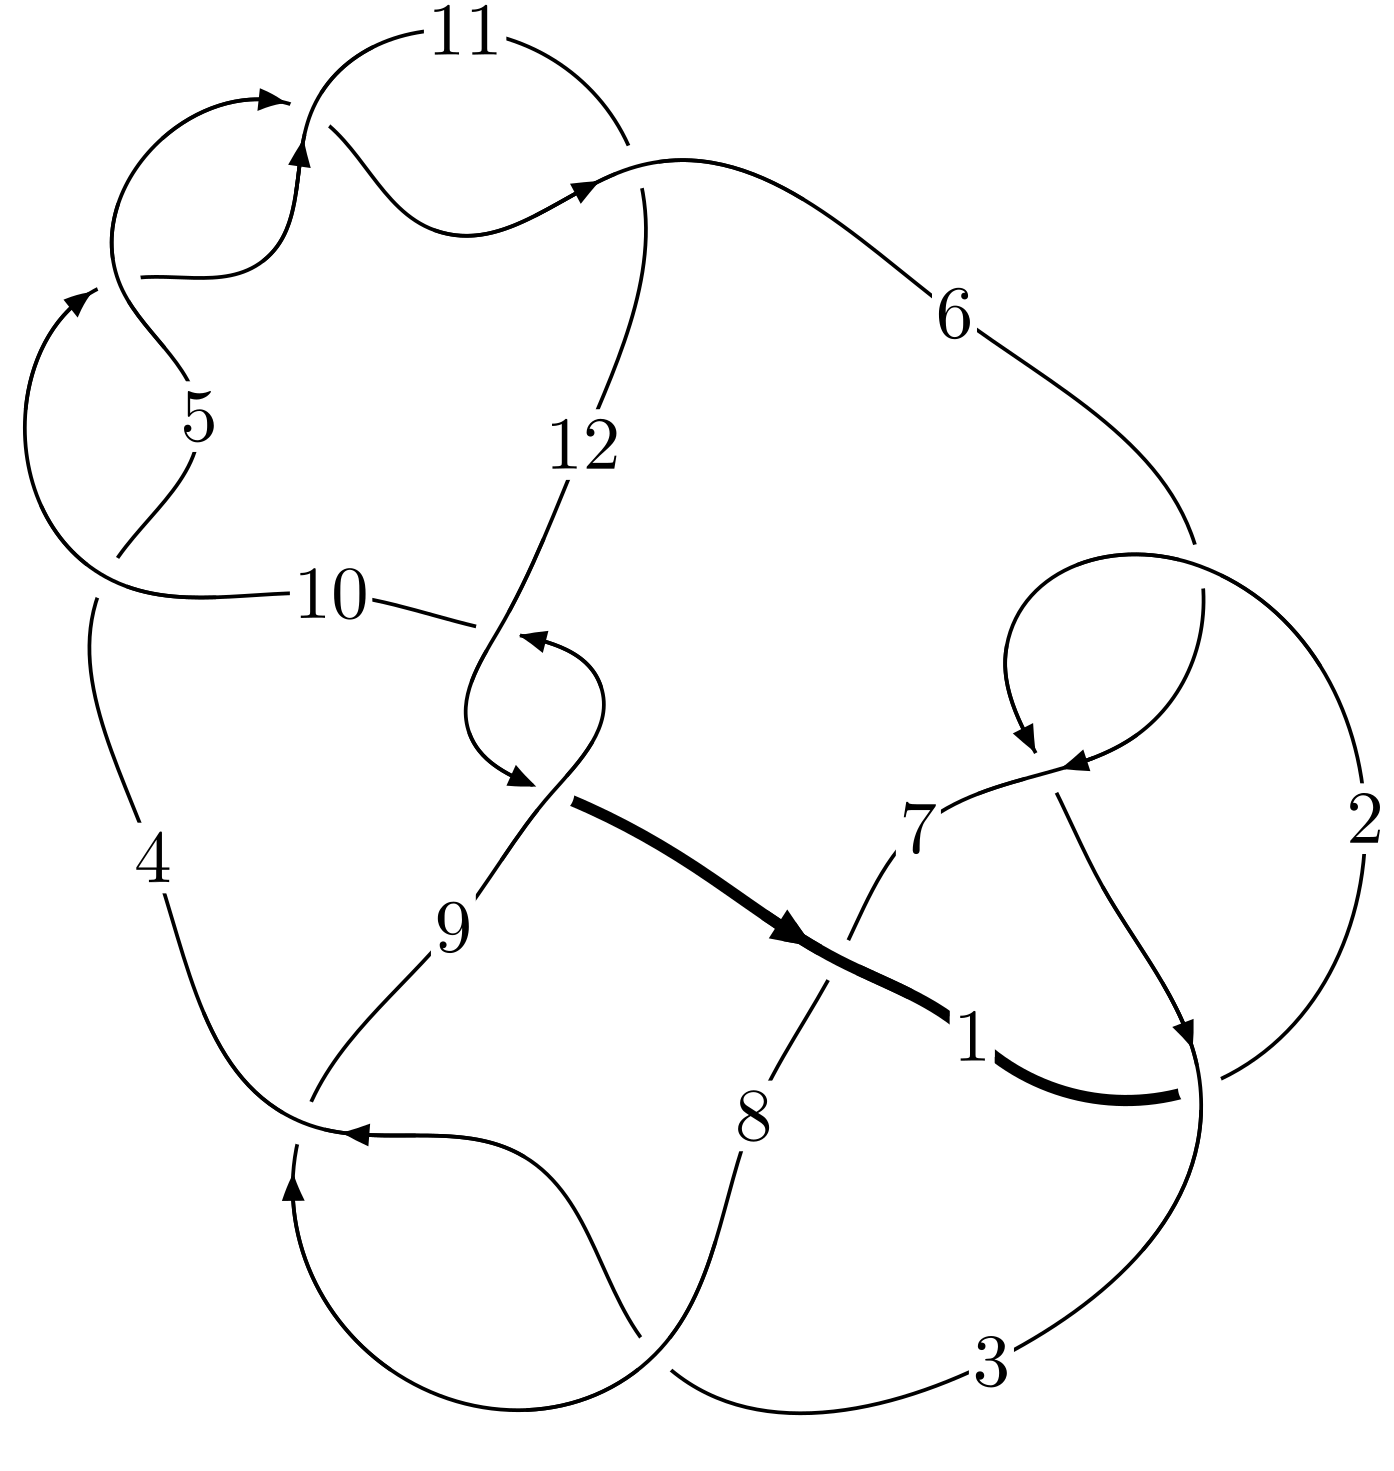
\includegraphics[width=112pt]{../../../GIT/diagram.site/Diagrams/png/1334_12a_0533.png}\\
\ \ \ A knot diagram\footnotemark}&
\allowdisplaybreaks
\textbf{Linearized knot diagam} \\
\cline{2-2}
 &
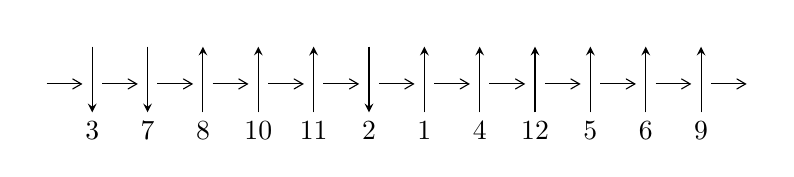
\begin{tikzpicture}[x=20pt, y=17pt]
	% nodes
	\node (C0) at (0, 0) {};
	\node (C1) at (1, 0) {};
	\node (C1U) at (1, +1) {};
	\node (C1D) at (1, -1) {3};

	\node (C2) at (2, 0) {};
	\node (C2U) at (2, +1) {};
	\node (C2D) at (2, -1) {7};

	\node (C3) at (3, 0) {};
	\node (C3U) at (3, +1) {};
	\node (C3D) at (3, -1) {8};

	\node (C4) at (4, 0) {};
	\node (C4U) at (4, +1) {};
	\node (C4D) at (4, -1) {10};

	\node (C5) at (5, 0) {};
	\node (C5U) at (5, +1) {};
	\node (C5D) at (5, -1) {11};

	\node (C6) at (6, 0) {};
	\node (C6U) at (6, +1) {};
	\node (C6D) at (6, -1) {2};

	\node (C7) at (7, 0) {};
	\node (C7U) at (7, +1) {};
	\node (C7D) at (7, -1) {1};

	\node (C8) at (8, 0) {};
	\node (C8U) at (8, +1) {};
	\node (C8D) at (8, -1) {4};

	\node (C9) at (9, 0) {};
	\node (C9U) at (9, +1) {};
	\node (C9D) at (9, -1) {12};

	\node (C10) at (10, 0) {};
	\node (C10U) at (10, +1) {};
	\node (C10D) at (10, -1) {5};

	\node (C11) at (11, 0) {};
	\node (C11U) at (11, +1) {};
	\node (C11D) at (11, -1) {6};

	\node (C12) at (12, 0) {};
	\node (C12U) at (12, +1) {};
	\node (C12D) at (12, -1) {9};
	\node (C13) at (13, 0) {};

	% arrows
	\draw[->,>={angle 60}]
	(C0) edge (C1) (C1) edge (C2) (C2) edge (C3) (C3) edge (C4) (C4) edge (C5) (C5) edge (C6) (C6) edge (C7) (C7) edge (C8) (C8) edge (C9) (C9) edge (C10) (C10) edge (C11) (C11) edge (C12) (C12) edge (C13) ;	\draw[->,>=stealth]
	(C1U) edge (C1D) (C2U) edge (C2D) (C3D) edge (C3U) (C4D) edge (C4U) (C5D) edge (C5U) (C6U) edge (C6D) (C7D) edge (C7U) (C8D) edge (C8U) (C9D) edge (C9U) (C10D) edge (C10U) (C11D) edge (C11U) (C12D) edge (C12U) ;
	\end{tikzpicture} \\
\hhline{~~} \\& 
\textbf{Solving Sequence} \\ \cline{2-2} 
 &
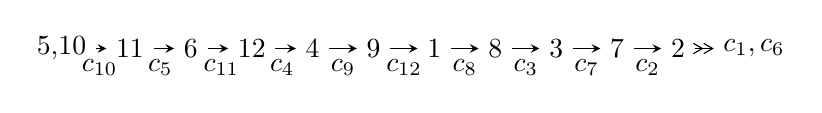
\begin{tikzpicture}[x=22pt, y=7pt]
	% node
	\node (A0) at (-1/8, 0) {5,10};
	\node (A1) at (1, 0) {11};
	\node (A2) at (2, 0) {6};
	\node (A3) at (3, 0) {12};
	\node (A4) at (4, 0) {4};
	\node (A5) at (5, 0) {9};
	\node (A6) at (6, 0) {1};
	\node (A7) at (7, 0) {8};
	\node (A8) at (8, 0) {3};
	\node (A9) at (9, 0) {7};
	\node (A10) at (10, 0) {2};
	\node (C1) at (1/2, -1) {$c_{10}$};
	\node (C2) at (3/2, -1) {$c_{5}$};
	\node (C3) at (5/2, -1) {$c_{11}$};
	\node (C4) at (7/2, -1) {$c_{4}$};
	\node (C5) at (9/2, -1) {$c_{9}$};
	\node (C6) at (11/2, -1) {$c_{12}$};
	\node (C7) at (13/2, -1) {$c_{8}$};
	\node (C8) at (15/2, -1) {$c_{3}$};
	\node (C9) at (17/2, -1) {$c_{7}$};
	\node (C10) at (19/2, -1) {$c_{2}$};
	\node (A11) at (45/4, 0) {$c_{1},c_{6}$};

	% edge
	\draw[->,>=stealth]	
	(A0) edge (A1) (A1) edge (A2) (A2) edge (A3) (A3) edge (A4) (A4) edge (A5) (A5) edge (A6) (A6) edge (A7) (A7) edge (A8) (A8) edge (A9) (A9) edge (A10) ;
	\draw[->>,>={angle 60}]	
	(A10) edge (A11);
\end{tikzpicture} \\ 

\end{tabular} \\

\footnotetext{
The image of knot diagram is generated by the software ``\textbf{Draw programme}" developed by Andrew Bartholomew(\url{http://www.layer8.co.uk/maths/draw/index.htm\#Running-draw}), where we modified some parts for our purpose(\url{https://github.com/CATsTAILs/LinksPainter}).
}\phantom \\ \newline 
\centering \textbf{Ideals for irreducible components\footnotemark of $X_{\text{par}}$} 
 
\begin{align*}
I^u_{1}&=\langle 
u^{68}+u^{67}+\cdots+3 u^2-1\rangle \\
\\
\end{align*}
\raggedright * 1 irreducible components of $\dim_{\mathbb{C}}=0$, with total 68 representations.\\
\footnotetext{All coefficients of polynomials are rational numbers. But the coefficients are sometimes approximated in decimal forms when there is not enough margin.}
\newpage
\renewcommand{\arraystretch}{1}
\centering \section*{I. $I^u_{1}= \langle u^{68}+u^{67}+\cdots+3 u^2-1 \rangle$}
\flushleft \textbf{(i) Arc colorings}\\
\begin{tabular}{m{7pt} m{180pt} m{7pt} m{180pt} }
\flushright $a_{5}=$&$\begin{pmatrix}0\\u\end{pmatrix}$ \\
\flushright $a_{10}=$&$\begin{pmatrix}1\\0\end{pmatrix}$ \\
\flushright $a_{11}=$&$\begin{pmatrix}1\\- u^2\end{pmatrix}$ \\
\flushright $a_{6}=$&$\begin{pmatrix}u\\- u^3+u\end{pmatrix}$ \\
\flushright $a_{12}=$&$\begin{pmatrix}- u^2+1\\u^4-2 u^2\end{pmatrix}$ \\
\flushright $a_{4}=$&$\begin{pmatrix}- u\\u\end{pmatrix}$ \\
\flushright $a_{9}=$&$\begin{pmatrix}- u^6+3 u^4-2 u^2+1\\u^8-4 u^6+4 u^4\end{pmatrix}$ \\
\flushright $a_{1}=$&$\begin{pmatrix}- u^{10}+5 u^8-8 u^6+5 u^4-3 u^2+1\\u^{12}-6 u^{10}+12 u^8-8 u^6+u^4-2 u^2\end{pmatrix}$ \\
\flushright $a_{8}=$&$\begin{pmatrix}- u^{10}+5 u^8-8 u^6+5 u^4-3 u^2+1\\u^{10}-4 u^8+3 u^6+2 u^4+u^2\end{pmatrix}$ \\
\flushright $a_{3}=$&$\begin{pmatrix}u^{19}-10 u^{17}+40 u^{15}-82 u^{13}+95 u^{11}-72 u^9+44 u^7-18 u^5+5 u^3-2 u\\- u^{19}+9 u^{17}-30 u^{15}+43 u^{13}-21 u^{11}+u^9-6 u^7- u^3+u\end{pmatrix}$ \\
\flushright $a_{7}=$&$\begin{pmatrix}u^{32}-17 u^{30}+\cdots-6 u^2+1\\- u^{34}+18 u^{32}+\cdots+8 u^4+u^2\end{pmatrix}$ \\
\flushright $a_{2}=$&$\begin{pmatrix}- u^{50}+27 u^{48}+\cdots-5 u^2+1\\u^{50}-26 u^{48}+\cdots-8 u^4- u^2\end{pmatrix}$\\&\end{tabular}
\flushleft \textbf{(ii) Obstruction class $= -1$}\\~\\
\flushleft \textbf{(iii) Cusp Shapes $= 4 u^{65}-144 u^{63}+\cdots-20 u+6$}\\~\\
\newpage\renewcommand{\arraystretch}{1}
\flushleft \textbf{(iv) u-Polynomials at the component}\newline \\
\begin{tabular}{m{50pt}|m{274pt}}
Crossings & \hspace{64pt}u-Polynomials at each crossing \\
\hline $$\begin{aligned}c_{1}\end{aligned}$$&$\begin{aligned}
&u^{68}+31 u^{67}+\cdots+6 u+1
\end{aligned}$\\
\hline $$\begin{aligned}c_{2},c_{6}\end{aligned}$$&$\begin{aligned}
&u^{68}- u^{67}+\cdots+2 u-1
\end{aligned}$\\
\hline $$\begin{aligned}c_{3},c_{8}\end{aligned}$$&$\begin{aligned}
&u^{68}+u^{67}+\cdots+92 u-13
\end{aligned}$\\
\hline $$\begin{aligned}c_{4},c_{5},c_{10}\\c_{11}\end{aligned}$$&$\begin{aligned}
&u^{68}- u^{67}+\cdots+3 u^2-1
\end{aligned}$\\
\hline $$\begin{aligned}c_{7}\end{aligned}$$&$\begin{aligned}
&u^{68}-3 u^{67}+\cdots-20 u+1
\end{aligned}$\\
\hline $$\begin{aligned}c_{9},c_{12}\end{aligned}$$&$\begin{aligned}
&u^{68}+13 u^{67}+\cdots-180 u-23
\end{aligned}$\\
\hline
\end{tabular}\\~\\
\newpage\renewcommand{\arraystretch}{1}
\flushleft \textbf{(v) Riley Polynomials at the component}\newline \\
\begin{tabular}{m{50pt}|m{274pt}}
Crossings & \hspace{64pt}Riley Polynomials at each crossing \\
\hline $$\begin{aligned}c_{1}\end{aligned}$$&$\begin{aligned}
&y^{68}+13 y^{67}+\cdots-6 y+1
\end{aligned}$\\
\hline $$\begin{aligned}c_{2},c_{6}\end{aligned}$$&$\begin{aligned}
&y^{68}-31 y^{67}+\cdots-6 y+1
\end{aligned}$\\
\hline $$\begin{aligned}c_{3},c_{8}\end{aligned}$$&$\begin{aligned}
&y^{68}-47 y^{67}+\cdots-9686 y+169
\end{aligned}$\\
\hline $$\begin{aligned}c_{4},c_{5},c_{10}\\c_{11}\end{aligned}$$&$\begin{aligned}
&y^{68}-75 y^{67}+\cdots-6 y+1
\end{aligned}$\\
\hline $$\begin{aligned}c_{7}\end{aligned}$$&$\begin{aligned}
&y^{68}+5 y^{67}+\cdots-110 y+1
\end{aligned}$\\
\hline $$\begin{aligned}c_{9},c_{12}\end{aligned}$$&$\begin{aligned}
&y^{68}+33 y^{67}+\cdots+7114 y+529
\end{aligned}$\\
\hline
\end{tabular}\\~\\
\newpage\flushleft \textbf{(vi) Complex Volumes and Cusp Shapes}
$$\begin{array}{c|c|c}  
\text{Solutions to }I^u_{1}& \I (\text{vol} + \sqrt{-1}CS) & \text{Cusp shape}\\
 \hline 
\begin{aligned}
u &= -0.835401 + 0.076969 I\end{aligned}
 & \phantom{-}3.98870 - 6.35660 I & \phantom{-}11.96357 + 5.97351 I \\ \hline\begin{aligned}
u &= -0.835401 - 0.076969 I\end{aligned}
 & \phantom{-}3.98870 + 6.35660 I & \phantom{-}11.96357 - 5.97351 I \\ \hline\begin{aligned}
u &= \phantom{-}0.831050 + 0.041295 I\end{aligned}
 & \phantom{-}5.76628 + 1.28729 I & \phantom{-}15.0699 - 0.8084 I \\ \hline\begin{aligned}
u &= \phantom{-}0.831050 - 0.041295 I\end{aligned}
 & \phantom{-}5.76628 - 1.28729 I & \phantom{-}15.0699 + 0.8084 I \\ \hline\begin{aligned}
u &= \phantom{-}0.612556 + 0.561591 I\end{aligned}
 & \phantom{-}0.04182 + 11.86150 I & \phantom{-}6.37979 - 10.46070 I \\ \hline\begin{aligned}
u &= \phantom{-}0.612556 - 0.561591 I\end{aligned}
 & \phantom{-}0.04182 - 11.86150 I & \phantom{-}6.37979 + 10.46070 I \\ \hline\begin{aligned}
u &= -0.612136 + 0.551160 I\end{aligned}
 & \phantom{-}2.09389 - 6.71465 I & \phantom{-}9.52044 + 6.37548 I \\ \hline\begin{aligned}
u &= -0.612136 - 0.551160 I\end{aligned}
 & \phantom{-}2.09389 + 6.71465 I & \phantom{-}9.52044 - 6.37548 I \\ \hline\begin{aligned}
u &= -0.616362 + 0.518645 I\end{aligned}
 & \phantom{-}2.80869 - 4.10090 I & \phantom{-}10.70764 + 6.36642 I \\ \hline\begin{aligned}
u &= -0.616362 - 0.518645 I\end{aligned}
 & \phantom{-}2.80869 + 4.10090 I & \phantom{-}10.70764 - 6.36642 I \\ \hline\begin{aligned}
u &= \phantom{-}0.585980 + 0.550245 I\end{aligned}
 & -2.78920 + 4.53214 I & \phantom{-}2.74588 - 5.66472 I \\ \hline\begin{aligned}
u &= \phantom{-}0.585980 - 0.550245 I\end{aligned}
 & -2.78920 - 4.53214 I & \phantom{-}2.74588 + 5.66472 I \\ \hline\begin{aligned}
u &= \phantom{-}0.621345 + 0.497725 I\end{aligned}
 & \phantom{-}1.38303 - 0.91928 I & \phantom{-}8.53731 - 1.06257 I \\ \hline\begin{aligned}
u &= \phantom{-}0.621345 - 0.497725 I\end{aligned}
 & \phantom{-}1.38303 + 0.91928 I & \phantom{-}8.53731 + 1.06257 I \\ \hline\begin{aligned}
u &= -0.507777 + 0.569607 I\end{aligned}
 & -5.47539 - 5.67160 I & \phantom{-}0.47362 + 7.79451 I \\ \hline\begin{aligned}
u &= -0.507777 - 0.569607 I\end{aligned}
 & -5.47539 + 5.67160 I & \phantom{-}0.47362 - 7.79451 I \\ \hline\begin{aligned}
u &= -0.464449 + 0.572539 I\end{aligned}
 & -5.60242 + 1.75390 I & -0.214027 - 0.465353 I \\ \hline\begin{aligned}
u &= -0.464449 - 0.572539 I\end{aligned}
 & -5.60242 - 1.75390 I & -0.214027 + 0.465353 I \\ \hline\begin{aligned}
u &= \phantom{-}0.486921 + 0.541642 I\end{aligned}
 & -2.59155 + 1.87214 I & \phantom{-}4.19602 - 4.04466 I \\ \hline\begin{aligned}
u &= \phantom{-}0.486921 - 0.541642 I\end{aligned}
 & -2.59155 - 1.87214 I & \phantom{-}4.19602 + 4.04466 I \\ \hline\begin{aligned}
u &= -0.694797\phantom{ +0.000000I}\end{aligned}
 & \phantom{-}0.907173\phantom{ +0.000000I} & \phantom{-}9.94330\phantom{ +0.000000I} \\ \hline\begin{aligned}
u &= \phantom{-}0.332805 + 0.598999 I\end{aligned}
 & -0.77445 - 7.89771 I & \phantom{-}4.14994 + 4.52279 I \\ \hline\begin{aligned}
u &= \phantom{-}0.332805 - 0.598999 I\end{aligned}
 & -0.77445 + 7.89771 I & \phantom{-}4.14994 - 4.52279 I \\ \hline\begin{aligned}
u &= \phantom{-}0.366988 + 0.568928 I\end{aligned}
 & -3.42846 - 0.68233 I & \phantom{-}0.547475 - 0.922163 I \\ \hline\begin{aligned}
u &= \phantom{-}0.366988 - 0.568928 I\end{aligned}
 & -3.42846 + 0.68233 I & \phantom{-}0.547475 + 0.922163 I \\ \hline\begin{aligned}
u &= -0.325745 + 0.583572 I\end{aligned}
 & \phantom{-}1.26237 + 2.82639 I & \phantom{-}7.27704 - 0.30320 I \\ \hline\begin{aligned}
u &= -0.325745 - 0.583572 I\end{aligned}
 & \phantom{-}1.26237 - 2.82639 I & \phantom{-}7.27704 + 0.30320 I \\ \hline\begin{aligned}
u &= \phantom{-}0.556194 + 0.317442 I\end{aligned}
 & -0.21535 + 3.63596 I & \phantom{-}8.68786 - 8.76844 I \\ \hline\begin{aligned}
u &= \phantom{-}0.556194 - 0.317442 I\end{aligned}
 & -0.21535 - 3.63596 I & \phantom{-}8.68786 + 8.76844 I \\ \hline\begin{aligned}
u &= -0.285763 + 0.538664 I\end{aligned}
 & \phantom{-}1.87263 + 0.44543 I & \phantom{-}8.05642 + 0.19579 I\\
 \hline 
 \end{array}$$\newpage$$\begin{array}{c|c|c}  
\text{Solutions to }I^u_{1}& \I (\text{vol} + \sqrt{-1}CS) & \text{Cusp shape}\\
 \hline 
\begin{aligned}
u &= -0.285763 - 0.538664 I\end{aligned}
 & \phantom{-}1.87263 - 0.44543 I & \phantom{-}8.05642 - 0.19579 I \\ \hline\begin{aligned}
u &= \phantom{-}0.244521 + 0.522979 I\end{aligned}
 & \phantom{-}0.33376 + 4.43660 I & \phantom{-}5.03394 - 5.63421 I \\ \hline\begin{aligned}
u &= \phantom{-}0.244521 - 0.522979 I\end{aligned}
 & \phantom{-}0.33376 - 4.43660 I & \phantom{-}5.03394 + 5.63421 I \\ \hline\begin{aligned}
u &= -1.43293 + 0.08268 I\end{aligned}
 & \phantom{-}4.69332 + 5.60280 I & \phantom{-0.000000 } 0 \\ \hline\begin{aligned}
u &= -1.43293 - 0.08268 I\end{aligned}
 & \phantom{-}4.69332 - 5.60280 I & \phantom{-0.000000 } 0 \\ \hline\begin{aligned}
u &= \phantom{-}1.45312 + 0.06829 I\end{aligned}
 & \phantom{-}6.74595 - 0.72677 I & \phantom{-0.000000 } 0 \\ \hline\begin{aligned}
u &= \phantom{-}1.45312 - 0.06829 I\end{aligned}
 & \phantom{-}6.74595 + 0.72677 I & \phantom{-0.000000 } 0 \\ \hline\begin{aligned}
u &= -0.524220 + 0.080652 I\end{aligned}
 & \phantom{-}0.800382 - 0.035159 I & \phantom{-}12.87268 + 1.03494 I \\ \hline\begin{aligned}
u &= -0.524220 - 0.080652 I\end{aligned}
 & \phantom{-}0.800382 + 0.035159 I & \phantom{-}12.87268 - 1.03494 I \\ \hline\begin{aligned}
u &= -1.46881 + 0.10794 I\end{aligned}
 & \phantom{-}2.45112 - 1.55036 I & \phantom{-0.000000 } 0 \\ \hline\begin{aligned}
u &= -1.46881 - 0.10794 I\end{aligned}
 & \phantom{-}2.45112 + 1.55036 I & \phantom{-0.000000 } 0 \\ \hline\begin{aligned}
u &= \phantom{-}1.50453 + 0.15035 I\end{aligned}
 & \phantom{-}0.861268 + 0.774157 I & \phantom{-0.000000 } 0 \\ \hline\begin{aligned}
u &= \phantom{-}1.50453 - 0.15035 I\end{aligned}
 & \phantom{-}0.861268 - 0.774157 I & \phantom{-0.000000 } 0 \\ \hline\begin{aligned}
u &= -1.52221 + 0.14559 I\end{aligned}
 & \phantom{-}4.06744 - 4.28308 I & \phantom{-0.000000 } 0 \\ \hline\begin{aligned}
u &= -1.52221 - 0.14559 I\end{aligned}
 & \phantom{-}4.06744 + 4.28308 I & \phantom{-0.000000 } 0 \\ \hline\begin{aligned}
u &= \phantom{-}1.52815 + 0.06626 I\end{aligned}
 & \phantom{-}7.60675 + 0.77642 I & \phantom{-0.000000 } 0 \\ \hline\begin{aligned}
u &= \phantom{-}1.52815 - 0.06626 I\end{aligned}
 & \phantom{-}7.60675 - 0.77642 I & \phantom{-0.000000 } 0 \\ \hline\begin{aligned}
u &= \phantom{-}1.52367 + 0.16029 I\end{aligned}
 & \phantom{-}1.24045 + 8.26818 I & \phantom{-0.000000 } 0 \\ \hline\begin{aligned}
u &= \phantom{-}1.52367 - 0.16029 I\end{aligned}
 & \phantom{-}1.24045 - 8.26818 I & \phantom{-0.000000 } 0 \\ \hline\begin{aligned}
u &= -1.54603 + 0.09488 I\end{aligned}
 & \phantom{-}6.83939 - 5.14255 I & \phantom{-0.000000 } 0 \\ \hline\begin{aligned}
u &= -1.54603 - 0.09488 I\end{aligned}
 & \phantom{-}6.83939 + 5.14255 I & \phantom{-0.000000 } 0 \\ \hline\begin{aligned}
u &= -1.55970 + 0.16290 I\end{aligned}
 & \phantom{-}4.38474 - 7.12790 I & \phantom{-0.000000 } 0 \\ \hline\begin{aligned}
u &= -1.55970 - 0.16290 I\end{aligned}
 & \phantom{-}4.38474 + 7.12790 I & \phantom{-0.000000 } 0 \\ \hline\begin{aligned}
u &= \phantom{-}1.56912 + 0.16482 I\end{aligned}
 & \phantom{-}9.39965 + 9.33939 I & \phantom{-0.000000 } 0 \\ \hline\begin{aligned}
u &= \phantom{-}1.56912 - 0.16482 I\end{aligned}
 & \phantom{-}9.39965 - 9.33939 I & \phantom{-0.000000 } 0 \\ \hline\begin{aligned}
u &= -1.56899 + 0.16875 I\end{aligned}
 & \phantom{-}7.3423 - 14.5405 I & \phantom{-0.000000 } 0 \\ \hline\begin{aligned}
u &= -1.56899 - 0.16875 I\end{aligned}
 & \phantom{-}7.3423 + 14.5405 I & \phantom{-0.000000 } 0 \\ \hline\begin{aligned}
u &= \phantom{-}1.57101 + 0.15333 I\end{aligned}
 & \phantom{-}10.15460 + 6.56396 I & \phantom{-0.000000 } 0 \\ \hline\begin{aligned}
u &= \phantom{-}1.57101 - 0.15333 I\end{aligned}
 & \phantom{-}10.15460 - 6.56396 I & \phantom{-0.000000 } 0 \\ \hline\begin{aligned}
u &= -1.57221 + 0.14666 I\end{aligned}
 & \phantom{-}8.75910 - 1.44505 I & \phantom{-0.000000 } 0\\
 \hline 
 \end{array}$$\newpage$$\begin{array}{c|c|c}  
\text{Solutions to }I^u_{1}& \I (\text{vol} + \sqrt{-1}CS) & \text{Cusp shape}\\
 \hline 
\begin{aligned}
u &= -1.57221 - 0.14666 I\end{aligned}
 & \phantom{-}8.75910 + 1.44505 I & \phantom{-0.000000 } 0 \\ \hline\begin{aligned}
u &= \phantom{-}1.58883\phantom{ +0.000000I}\end{aligned}
 & \phantom{-}8.73667\phantom{ +0.000000I} & \phantom{-0.000000 } 0 \\ \hline\begin{aligned}
u &= -1.60657 + 0.00745 I\end{aligned}
 & \phantom{-}14.01720 - 1.44111 I & \phantom{-0.000000 } 0 \\ \hline\begin{aligned}
u &= -1.60657 - 0.00745 I\end{aligned}
 & \phantom{-}14.01720 + 1.44111 I & \phantom{-0.000000 } 0 \\ \hline\begin{aligned}
u &= \phantom{-}1.60735 + 0.01384 I\end{aligned}
 & \phantom{-}12.25660 + 6.64311 I & \phantom{-0.000000 } 0 \\ \hline\begin{aligned}
u &= \phantom{-}1.60735 - 0.01384 I\end{aligned}
 & \phantom{-}12.25660 - 6.64311 I & \phantom{-0.000000 } 0 \\ \hline\begin{aligned}
u &= \phantom{-}0.106973 + 0.377298 I\end{aligned}
 & -1.48571 - 1.30445 I & \phantom{-}0.644293 + 0.844711 I \\ \hline\begin{aligned}
u &= \phantom{-}0.106973 - 0.377298 I\end{aligned}
 & -1.48571 + 1.30445 I & \phantom{-}0.644293 - 0.844711 I\\
 \hline 
 \end{array}$$\newpage
\newpage\renewcommand{\arraystretch}{1}
\centering \section*{ II. u-Polynomials}
\begin{tabular}{m{50pt}|m{274pt}}
Crossings & \hspace{64pt}u-Polynomials at each crossing \\
\hline $$\begin{aligned}c_{1}\end{aligned}$$&$\begin{aligned}
&u^{68}+31 u^{67}+\cdots+6 u+1
\end{aligned}$\\
\hline $$\begin{aligned}c_{2},c_{6}\end{aligned}$$&$\begin{aligned}
&u^{68}- u^{67}+\cdots+2 u-1
\end{aligned}$\\
\hline $$\begin{aligned}c_{3},c_{8}\end{aligned}$$&$\begin{aligned}
&u^{68}+u^{67}+\cdots+92 u-13
\end{aligned}$\\
\hline $$\begin{aligned}c_{4},c_{5},c_{10}\\c_{11}\end{aligned}$$&$\begin{aligned}
&u^{68}- u^{67}+\cdots+3 u^2-1
\end{aligned}$\\
\hline $$\begin{aligned}c_{7}\end{aligned}$$&$\begin{aligned}
&u^{68}-3 u^{67}+\cdots-20 u+1
\end{aligned}$\\
\hline $$\begin{aligned}c_{9},c_{12}\end{aligned}$$&$\begin{aligned}
&u^{68}+13 u^{67}+\cdots-180 u-23
\end{aligned}$\\
\hline
\end{tabular}\newpage\renewcommand{\arraystretch}{1}
\centering \section*{ III. Riley Polynomials}
\begin{tabular}{m{50pt}|m{274pt}}
Crossings & \hspace{64pt}Riley Polynomials at each crossing \\
\hline $$\begin{aligned}c_{1}\end{aligned}$$&$\begin{aligned}
&y^{68}+13 y^{67}+\cdots-6 y+1
\end{aligned}$\\
\hline $$\begin{aligned}c_{2},c_{6}\end{aligned}$$&$\begin{aligned}
&y^{68}-31 y^{67}+\cdots-6 y+1
\end{aligned}$\\
\hline $$\begin{aligned}c_{3},c_{8}\end{aligned}$$&$\begin{aligned}
&y^{68}-47 y^{67}+\cdots-9686 y+169
\end{aligned}$\\
\hline $$\begin{aligned}c_{4},c_{5},c_{10}\\c_{11}\end{aligned}$$&$\begin{aligned}
&y^{68}-75 y^{67}+\cdots-6 y+1
\end{aligned}$\\
\hline $$\begin{aligned}c_{7}\end{aligned}$$&$\begin{aligned}
&y^{68}+5 y^{67}+\cdots-110 y+1
\end{aligned}$\\
\hline $$\begin{aligned}c_{9},c_{12}\end{aligned}$$&$\begin{aligned}
&y^{68}+33 y^{67}+\cdots+7114 y+529
\end{aligned}$\\
\hline
\end{tabular}
\vskip 2pc
\end{document}